\documentclass[border=2pt]{standalone}
\usepackage{tikz}
\usetikzlibrary{arrows.meta,topaths}

\begin{document}
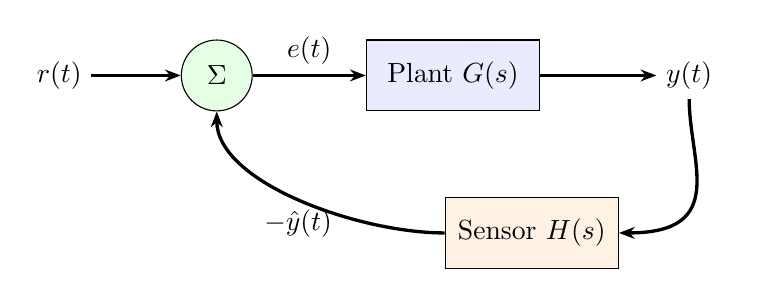
\begin{tikzpicture}[
  block/.style={draw,minimum width=22mm,minimum height=9mm,align=center},
  signal/.style={-{Stealth[length=2mm]},very thick}
]
  \node (reference) at (0,0) {$r(t)$};
  \node[draw,circle,minimum size=9mm,fill=green!10] (sum) at (2,0) {$\Sigma$};
  \node[block,fill=blue!8] (plant) at (5,0) {Plant $G(s)$};
  \node (output) at (8,0) {$y(t)$};
  \node[block,fill=orange!10] (sensor) at (6,-2) {Sensor $H(s)$};

  \path[signal]
    (reference) edge (sum)
    (sum) edge node[above] {$e(t)$} (plant)
    (plant) edge (output)
    (output) edge[out=-90,in=0,out distance=8mm,in distance=14mm] (sensor)
    (sensor) edge[
      out=180,
      in=-90,
      out looseness=.35,
      in looseness=2,
      out min distance=11mm,
      in max distance=9mm
    ] node[below] {$-\hat y(t)$} (sum);
\end{tikzpicture}
\end{document}
